\chapter{实验概述}
\label{cha:shi_yan_gai_shu_}

\section{源语言定义}
\label{sec:yuan_yu_yan_ding_yi_}

\par 本实验实现了一个Decaf语言的编译器。Decaf/Mind 是一种强类型的面向对象的、支持继承和封装的语言,此语言与C/C++十分类似,但并不完全一样。本实验中实现的Decaf语言采用了TAMU CS434的Decaf语言定义\footnote{\url{https://parasol.tamu.edu/courses/decaf/students/decafOverview.pdf}}。

\section{实验内容}
\label{sec:shi_yan_nei_rong_}

\par 本次实验实现的程序按照内容分为以下几个部分:
\begin{itemize}
    \item 实验一:词法语法分析器的设计与实现:词法分析工具使用Flex,语法分析工具使用bison完成。
    \item 实验二:语义分析以及符号表的设计与计算:生成抽象语法树,进行语义分析,设计符号表数据结构和关键管理功能。动态展现符号表变化过程。
    \item 实验三:中间代码生成:实现类型检查和控制语句目标地址计算,生成中间代码。
    \item 实验四:目标代码生成:在前三个实验的基础上实现MIPS平台目标代码生成。
\end{itemize}

\section{实验环境}
\label{sec:shi_yan_huan_jing_}

\par 本次实验在如表\ref{tab:environment}所示的环境下进行。
\begin{table}[htbp]
    \centering
    \caption{实验环境}
    \label{tab:environment}
    \begin{tabular}{r l}
        \toprule
        \multicolumn{1}{c}{\textbf{环境}} &
        \multicolumn{1}{c}{\textbf{版本}} \\
        \cmidrule(lr){1-1} \cmidrule(lr){2-2}
        操作系统    & Arch Linux 2018-06-10 更新\\
        flex        & 2.6.4 \\
        bison       & 3.0.5 \\
        gcc         & 8.1.1 \\
        mips模拟器  & Mars 4.5 \\
        \bottomrule
    \end{tabular}
\end{table}

\chapter{词法分析与语法分析}
\label{cha:ci_fa_fen_xi_yu_yu_fa_fen_xi_}

\section{实验设计}
\label{sec:shi_yan_she_ji_1}
\par 为了便于程序的设计,以及基于逻辑上的原因,在这一部分中首先编写用于语法分析的程序,然后根据此程序编写用于词法分析的程序。

\par 首先,按照语法定义列出所有的终结符以及非终结符,如表\ref{tab:tokens}所示,然后定义运算符的优先级与结合性,如表\ref{tab:priority}所示,最后按照语法规则完成bison的EBNF的编写。语法规则在\ref{sec:yuan_yu_yan_ding_yi_}一节中已经给出。

\begin{table}[htbp]
    \centering
    \caption{语法符号}
    \label{tab:tokens}
    \begin{tabu} to 0.8\textwidth {X[2] X}
        \toprule
        \multicolumn{1}{c}{\textbf{符号}} &
        \multicolumn{1}{c}{\textbf{说明}} \\
        \cmidrule(lr){1-1} \cmidrule(lr){2-2}
        tokenVoid tokenBool tokenInt tokenDouble tokenString tokenClass & 终结符:变量类型关键字 \\ \cmidrule(lr){1-2}
        tokenLessEqual tokenGreaterEqual tokenEqual tokenNotEqual tokenDims & 终结符:二元运算符 \\ \cmidrule(lr){1-2}
        tokenAnd tokenOr tokenNull tokenExtends tokenThis tokenInterface tokenImplements & 终结符:逻辑运算符以及类相关运算符 \\ \cmidrule(lr){1-2}
        tokenWhile tokenFor tokenIf tokenElse tokenReturn tokenBreak & 终结符:流程控制关键字 \\ \cmidrule(lr){1-2}
        tokenNew tokenNewArray tokenPrint tokenReadInteger tokenReadLine & 终结符:内建函数关键字 \\ \cmidrule(lr){1-2}
        tokenIdentifier tokenStringConstant tokenIntConstant tokenDoubleConstant tokenBoolConstant & 终结符:常量 \\ \cmidrule(lr){1-2}
        Constant Expr Call OptExpr LValue Type OptExt OptImpl ImpList ClassDecl Decl Field IntfDecl FnDecl FnHeader FieldList DeclList IntfList Variable VarDecl Formals FormalList VarDecls Actuals ExprList Stmt StmtBlock OptElse & 非终结符 \\
        \bottomrule
    \end{tabu}
\end{table}

\newcommand\tikzmark[2]{%
    \tikz[remember picture,baseline] \node[inner sep=2pt,outer sep=0] (#1){#2};%
}
\newcommand\link[2]{%
    \begin{tikzpicture}[remember picture, overlay, >=stealth, shift={(0,0)}]
        \draw[->] (#1) to (#2);
    \end{tikzpicture}%
}

\inputCodeNoNumberSetLanguage{[plain]TeX}
\begin{table}[htpb]
    \centering
    \caption{优先级与结合性}
    \label{tab:priority}
    \begin{tabular}{c c l}
        \toprule
        \multicolumn{1}{c}{\textbf{优先级}} &
        \multicolumn{1}{c}{\textbf{结合性}} &
        \multicolumn{1}{c}{\textbf{符号}} \\
        \cmidrule(lr){1-1} \cmidrule(lr){2-2} \cmidrule(lr){3-3}
        \tikzmark{a}{高} & 左结合 & \lstinline|'='| \\
                         & 左结合 & tokenOr \\
                         & 左结合 & tokenAnd \\
                         & 无     & tokenEqual tokenNotEqual \\
                         & 无     & \lstinline|'<'| \lstinline|`>'| tokenLessEqual tokenGreaterEqual \\
                         & 左结合 & \lstinline|'+'| \lstinline|'-'| \\
                         & 左结合 & \lstinline|'*'| \lstinline|'/'| \lstinline|'%'| \\
                         & 无     & tokenUnaryMinus \lstinline|'!'| \\
                         & 无     & \lstinline|'.'| \lstinline|'['| \\
                         & 无     & tokenLower\_Than\_Else \\
        \tikzmark{b}{低} & 无     & tokenElse \\
        \bottomrule
    \end{tabular}
    \link{a}{b}
\end{table}

\par 在进行bison语法分分析器的编写后,依照语法符号中的终结符给出词法的定义,并使用Flex编写词法分析器。其中,对于常量类型使用的正则表达式如表\ref{tab:regex}所示。
\inputCodeSetLanguage{[plain]TeX}
\begin{table}[htpb]
    \centering
    \caption{词法分析中的正则表达式}
    \label{tab:regex}
    \begin{tabular}{r l l}
        \toprule
        \multicolumn{1}{c}{\textbf{名称}} &
        \multicolumn{1}{c}{\textbf{正则表达式}} &
        \multicolumn{1}{c}{\textbf{说明}} \\
        \cmidrule(lr){1-1} \cmidrule(lr){2-2} \cmidrule(lr){3-3}
        integerHex          & \lstinline|(0[Xx][0-9a-fA-F]+)|               & 16进制整形\\
        integer             & \lstinline|([0-9]+)|                          & 10进制整形\\
        exponent            & \lstinline|([Ee][-+]?{integer\})|             & 科学记数法后缀\\
        double              & \lstinline|({integer}"."[0-9]*{exponent}?)|   & 浮点型\\
        stringBegin         & \lstinline|(\"[^"\n]*)|                       & 字符串开始\\
        string              & \lstinline|({stringBegin}\")|                 & 字符串\\
        identifier          & \lstinline|([a-zA-Z][a-zA-Z_0-9]*)|           & 标识符\\
        operator            & \lstinline|([-+/*%=.,;!<>()[\]{}])|           & 运算符\\
        commentBegin        & \lstinline|("/*")|                            & 注释开始\\
        commentEnd          & \lstinline|("*/")|                            & 注释结束\\
        commentSingleLine   & \lstinline|("//"[^\n]*)|                      & 单行注释\\
        \bottomrule
    \end{tabular}
\end{table}
\par 在扫描到每个token后首先进行输出,然后直接返回bison中已经定义好的token类型即可。此外,词法分析器中还定义了三个额外的状态:COMMON、COPY以及COMMENTS,这些状态用于帮助处理token的扫描。其中COPY状态用于复制远吗中的内容,便于后续的调试以及错误处理,NORMAL态为正常的词法分析状态,而COMMENTS态为程序处理注释时的状态,此时程序忽略其他所有的规则直到注释结束。程序初始时为COPY态,此后对于每一个token的扫描COPY态与NORMAL态交替出现,在复制源程序全部信息的同时完成对于词法的分析,输出以及传递给bison生成的程序。

\section{实验过程}
\label{sec:shi_yan_bu_zou_1}
\par 首先,按照实验设计中的语法规则编写bison以及flex程序(具体程序见附录\ref{cha:bian_yi_qi_yuan_dai_ma_})。然后使用bison和flex处理得到lex.yy.c以及y.tab.c。将生成的c程序进行编译和链接,得到可执行文件。此外,在使用bison的过程中会生成一个y.output文件,此文件为生成的语法分析器的状态机,可以利用这一文件以及bison的interactive mode对于状态机进行调试,以便于快速的检测出错误。
\par 连接得到可执行文件后,编写一个Decaf程序以用于测试,此处编写的是一个排序Decaf程序,将测试程序输入到得到的编译器中,生成分析结果文件后观察文件内容。

\section{实验结果及分析}
\label{sec:shi_yan_jie_guo_ji_fen_xi_1}

\par 输入测试程序1(见附录\ref{cha:ce_shi_yong_decafdai_ma_}),得到的词法分析输出如图\ref{fig:lexout}所示(未显示完全),然后将生成的Decaf程序与源程序进行比对,发现没有缺失或错误翻译的情况存在,初步说明词法分析程序实现了计划的功能。
\begin{figure}[htpb]
    \centering
    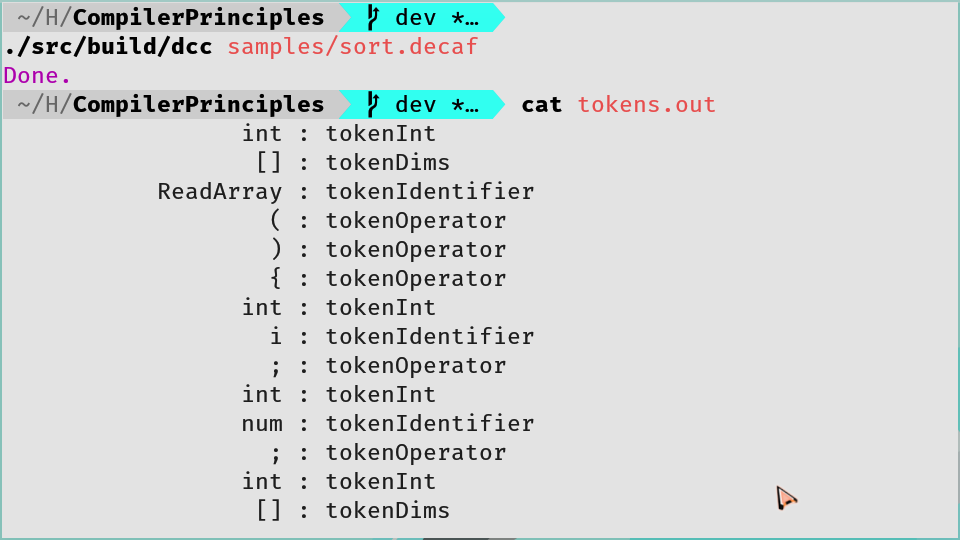
\includegraphics[width=0.8\linewidth]{lexout.png}
    \caption{词法分析输出}
    \label{fig:lexout}
\end{figure}

\par 对于语法分析而言,由于实验进行到此处时只制定了语法规则,而未指定对应的动作,因此只能初步通过编译信息保证这一bison程序本身没有语法错误,而不能保证其功能正确。在接下来的章节中,将继续完善语法分析程序的动作,构建语法树并将其输出,以完整的检测语法分析器的正确性。


